\documentclass{article}
\usepackage[utf8]{inputenc}
\usepackage[T5]{fontenc}
\usepackage{graphicx}
\usepackage{authblk}
\usepackage{amsmath} % Thêm gói này để viết công thức toán (A$^*$)
\usepackage{tikz}
\usetikzlibrary{shapes.misc, arrows.meta, positioning, quotes}
\usepackage{listings}
\usepackage{xcolor}

\definecolor{codegreen}{rgb}{0,0.6,0}
\definecolor{codegray}{rgb}{0.5,0.5,0.5}
\definecolor{codepurple}{rgb}{0.58,0,0.82}
\definecolor{backcolour}{rgb}{0.95,0.95,0.92}

\lstdefinestyle{mystyle}{
    backgroundcolor=\color{backcolour},
    commentstyle=\color{codegreen},
    keywordstyle=\color{magenta},
    numberstyle=\tiny\color{codegray},
    stringstyle=\color{codepurple},
    basicstyle=\footnotesize\ttfamily,
    breakatwhitespace=false,
    breaklines=true,
    captionpos=b,
    keepspaces=true,
    numbers=left,
    numbersep=5pt,
    showspaces=false,
    showstringspaces=false,
    showtabs=false,
    tabsize=2
}

\lstset{style=mystyle}

\title{Project 1: Search}

\author{Lê Mai Việt Hoàng}
\author{Nguyễn Đức Anh Tuấn}
\author{Lê Thị Hồng Hoa}

\affil{\textit{University of Engineering and Technology, VNU}}
\affil{Email: 22022191@vnu.edu.vn, 2302xxxx@vnu.edu.vn, 2202xxxx@vnu.edu.vn}

\date{December 2025}

\begin{document}

\maketitle

% ----------------------------------------------------------------------
% PHẦN 1: GIỚI THIỆU
% ----------------------------------------------------------------------
\section{Giới thiệu}

Trong lĩnh vực Trí tuệ Nhân tạo, các thuật toán tìm kiếm đóng vai trò nền tảng trong việc giải quyết đa dạng các bài toán, từ tìm đường đi (pathfinding) cho đến lập kế hoạch chiến lược. Báo cáo này trình bày quá trình cài đặt và phân tích kết quả của nhóm cho \textbf{Project 1: Search} thuộc khóa học CS 188 (Cơ sở trí tuệ nhân tạo). Mục tiêu chính của dự án là xây dựng các thuật toán tìm kiếm tổng quát và áp dụng chúng vào môi trường của trò chơi Pacman, cho phép tác tử (agent) định hướng di chuyển trong mê cung và thu thập thức ăn một cách hiệu quả.

Dự án được cấu trúc nhằm dẫn dắt người học từ các chiến lược tìm kiếm không có thông tin (uninformed search) đến các phương pháp tìm kiếm có thông tin (informed search) nâng cao hơn. Cụ thể, chúng tôi tập trung vào các nội dung chính được cài đặt trong các tệp \texttt{search.py} và \texttt{searchAgents.py} như sau:

\begin{itemize}
    \item \textbf{Tìm kiếm không có thông tin (Uninformed Search):} Nhóm thực hiện cài đặt các thuật toán Tìm kiếm theo chiều sâu (DFS), Tìm kiếm theo chiều rộng (BFS) và Tìm kiếm chi phí thống nhất (UCS). Các thuật toán này được thử nghiệm trên nhiều cấu trúc mê cung khác nhau (như \textit{tinyMaze, mediumMaze, bigMaze}) để đánh giá khả năng tìm đường cũng như tính tối ưu về chi phí.
    \item \textbf{Tìm kiếm có thông tin (Informed Search - A$^*$):} Chúng tôi cài đặt thuật toán tìm kiếm A$^*$ và phát triển các hàm heuristic tùy chỉnh. Phần này chứng minh cách tri thức đặc thù của miền bài toán (thông qua hàm heuristic) có thể giảm thiểu đáng kể không gian tìm kiếm cho các tác vụ phức tạp, ví dụ như \textit{Corners Problem} (đi qua 4 góc mê cung) và \textit{Food Search Problem} (ăn tất cả các chấm thức ăn).
    \item \textbf{Tìm kiếm gần tối ưu (Suboptimal Search):} Cuối cùng, báo cáo khảo sát các phương pháp tham lam (greedy approaches) cho các kịch bản mà việc tìm ra lời giải tối ưu tốn quá nhiều chi phí tính toán, nhằm cân bằng giữa chất lượng lời giải và thời gian thực thi.
\end{itemize}

Thông qua dự án này, nhóm mong muốn thể hiện sự hiểu biết vững chắc về cách các chiến lược tìm kiếm khác nhau ảnh hưởng đến hành vi của tác tử, số lượng nút được mở rộng (nodes expanded) và hiệu quả tổng thể.

% ----------------------------------------------------------------------
% PHẦN 2: CÁC CÔNG VIỆC LIÊN QUAN / CƠ SỞ LÝ THUYẾT
% ----------------------------------------------------------------------
\section{Cơ sở lý thuyết và Các công việc liên quan}

Để giải quyết bài toán Pacman, chúng tôi dựa trên mô hình bài toán tìm kiếm chuẩn (Standard Search Problem) và các cấu trúc dữ liệu cơ bản đã được học trong lý thuyết.

\subsection{Mô hình hóa bài toán tìm kiếm}
Một bài toán tìm kiếm có thể được định nghĩa hình thức bằng một bộ 5 thành phần $(S, s_{start}, A, T, Goal)$:

\begin{itemize}
    \item \textbf{Không gian trạng thái (State Space) $S$:} Tập hợp tất cả các trạng thái có thể xảy ra trong môi trường.
    \begin{itemize}
        \item \textit{Ví dụ:} Trong bài toán tìm đường đơn giản, $S$ là tập hợp các tọa độ lưới $(x, y)$. Trong \textit{CornersProblem}, trạng thái là một tuple $((x, y), (c_1, c_2, c_3, c_4))$ với $c_i \in \{0, 1\}$ biểu thị trạng thái đã thăm của 4 góc.
    \end{itemize}
    
    \item \textbf{Trạng thái bắt đầu $s_{start} \in S$:} Vị trí khởi tạo của Pacman.
    
    \item \textbf{Tập hành động $A(s)$:} Các hành động hợp lệ từ trạng thái $s$. Trong Pacman, $A = \{North, South, East, West, Stop\}$.
    
    \item \textbf{Hàm kế tiếp và Chi phí (Successor \& Cost):} Hàm trả về bộ ba $(s', a, c)$, trong đó $s'$ là trạng thái kế tiếp khi thực hiện hành động $a$ với chi phí $c$.
    \[ T(s, a) \rightarrow s' \]
    \[ Cost(s, a, s') \geq 0 \]
    Trong mê cung thông thường, chi phí cho mỗi bước di chuyển là $1$.
    
    \item \textbf{Kiểm tra đích (Goal Test):} Hàm boolean $Goal(s)$ trả về \texttt{True} nếu $s$ là trạng thái đích.
\end{itemize}

\subsection{Các chiến lược tìm kiếm (Search Strategies)}
Hiệu năng của các thuật toán được đánh giá qua 4 tiêu chí: tính đầy đủ (completeness), tính tối ưu (optimality), độ phức tạp thời gian (time complexity) và độ phức tạp không gian (space complexity). Gọi $b$ là hệ số nhánh (branching factor), $d$ là độ sâu của lời giải nông nhất, và $m$ là độ sâu tối đa của không gian trạng thái.

\subsubsection{Tìm kiếm không có thông tin (Uninformed Search)}
Các thuật toán này chỉ dựa vào cấu trúc đồ thị để duyệt mà không biết đích còn bao xa.

\begin{enumerate}
    \item \textbf{Depth First Search (DFS):}
    \begin{itemize}
        \item Nguyên lý: Mở rộng nút sâu nhất trong tập biên (fringe) hiện tại. Sử dụng cấu trúc \textbf{Stack (LIFO)}.
        \item Đặc điểm: Không đảm bảo tìm thấy đích (nếu không gian vô hạn) và không đảm bảo tối ưu.
        \item Độ phức tạp: Thời gian $O(b^m)$, Không gian $O(b \cdot m)$ (tiết kiệm bộ nhớ).
    \end{itemize}

    \item \textbf{Breadth First Search (BFS):}
    \begin{itemize}
        \item Nguyên lý: Mở rộng nút nông nhất. Sử dụng cấu trúc \textbf{Queue (FIFO)}.
        \item Đặc điểm: Đảm bảo tìm ra lời giải ngắn nhất (nếu các bước có chi phí bằng nhau).
        \item Độ phức tạp: Thời gian $O(b^d)$, Không gian $O(b^d)$ (tốn rất nhiều bộ nhớ).
    \end{itemize}

    \item \textbf{Uniform Cost Search (UCS):}
    \begin{itemize}
        \item Nguyên lý: Mở rộng nút có chi phí đường đi tích lũy $g(n)$ thấp nhất. Sử dụng \textbf{Priority Queue}.
        \item Đặc điểm: Đảm bảo tối ưu cho mọi loại chi phí dương.
        \item Công thức: Chọn nút $n$ sao cho $g(n) = \min_{n' \in Fringe} g(n')$.
    \end{itemize}
\end{enumerate}

\subsubsection{Tìm kiếm có thông tin (Informed Search - A$^*$)}
Thuật toán A$^*$ kết hợp chi phí thực tế $g(n)$ và hàm ước lượng heuristic $h(n)$ để định hướng tìm kiếm:
\begin{equation}
    f(n) = g(n) + h(n)
\end{equation}
Trong đó $h(n)$ ước lượng chi phí rẻ nhất từ nút $n$ đến đích.

\paragraph{Tính chất của hàm Heuristic:}
Để A$^*$ đảm bảo tìm ra lời giải tối ưu (Optimal), hàm $h(n)$ cần thỏa mãn:

\begin{itemize}
    \item \textbf{Tính chấp nhận được (Admissibility):} $h(n)$ không bao giờ đánh giá cao hơn chi phí thực tế $h^*(n)$ để đến đích.
    \[ 0 \leq h(n) \leq h^*(n), \quad \forall n \]
    \textit{Ví dụ:} Khoảng cách Manhattan là admissible vì Pacman không thể đi chéo, nên khoảng cách thực tế luôn lớn hơn hoặc bằng khoảng cách Manhattan.
    \[ h_{Manhattan}((x_1, y_1), (x_2, y_2)) = |x_1 - x_2| + |y_1 - y_2| \]
    
    \item \textbf{Tính nhất quán (Consistency):} Hiệu của heuristic giữa hai trạng thái kề nhau không được lớn hơn chi phí thực tế giữa chúng.
    \[ h(n) \leq c(n, a, n') + h(n') \]
    Tính chất này đảm bảo rằng khi A$^*$ tìm thấy một nút, đó là đường đi ngắn nhất đến nút đó.
\end{itemize}

\subsection{Ví dụ minh họa các thuật toán}
Để minh họa cách các thuật toán tìm kiếm hoạt động trong thực tế, chúng ta hãy xem xét một mê cung nhỏ đơn giản.
Mục tiêu là tìm đường đi từ ô bắt đầu \textbf{S} đến ô đích \textbf{G}. Các ô đen (\textbf{X}) là tường không thể đi qua.

\begin{figure}[h!]
    \centering
    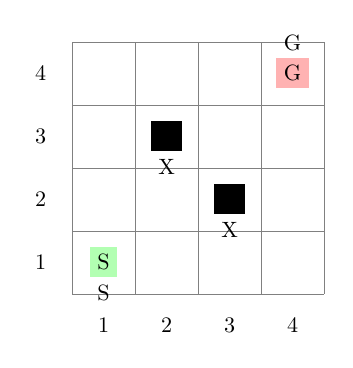
\begin{tikzpicture}[scale=0.8, every node/.style={scale=0.8}]
        % Grid
        \draw[step=1.0, gray, very thin] (0,0) grid (4,4);
        % Nodes
        \node[fill=green!30, label=below:S] at (0.5,0.5) {S};
        \node[fill=red!30, label=above:G] at (3.5,3.5) {G};
        \node[fill=black, label=below:X] at (1.5,2.5) {X};
        \node[fill=black, label=below:X] at (2.5,1.5) {X};
        % Coordinates
        \foreach \x in {1,...,4} {
            \node at (\x-0.5, -0.5) {\x};
        }
        \foreach \y in {1,...,4} {
            \node at (-0.5, \y-0.5) {\y};
        }
    \end{tikzpicture}
    \caption{Mê cung ví dụ. S là điểm bắt đầu (1,1), G là đích (4,4).}
    \label{fig:maze_example}
\end{figure}

Trong ví dụ này, chúng ta giả sử thứ tự duyệt các nút lân cận là: \textbf{Lên (Up), Xuống (Down), Trái (Left), Phải (Right)}.

\subsubsection{Depth First Search (DFS)}
DFS sẽ ưu tiên đi sâu nhất có thể. Lộ trình của nó có thể trông như sau:
\begin{itemize}
    \item \textbf{Tập biên (Stack):} [S]
    \item \textbf{Mở rộng S (1,1):} thêm các con (1,2), (2,1). Stack: [(1,2), (2,1)]
    \item \textbf{Mở rộng (1,2):} thêm (1,3). Stack: [(1,3), (2,1)]
    \item \textbf{Mở rộng (1,3):} thêm (1,4), (2,3) là tường. Stack: [(1,4), (2,1)]
    \item \textbf{Mở rộng (1,4):} thêm (2,4). Stack: [(2,4), (2,1)]
    \item ... và cứ thế tiếp tục.
\end{itemize}
DFS có thể tìm ra một đường đi rất dài và không hiệu quả trước khi tìm thấy đích. Ví dụ, nó có thể đi hết một nhánh rồi mới quay lại (backtrack).

\begin{figure}[h!]
    \centering
    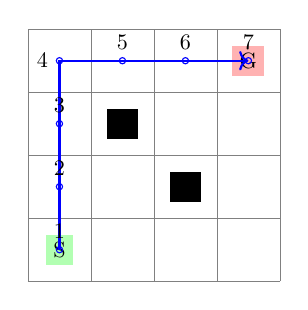
\begin{tikzpicture}[scale=0.8, every node/.style={scale=0.8}]
        % Grid
        \draw[step=1.0, gray, very thin] (0,0) grid (4,4);
        % Nodes
        \node[fill=green!30] at (0.5,0.5) {S};
        \node[fill=red!30] at (3.5,3.5) {G};
        \node[fill=black] at (1.5,2.5) {X};
        \node[fill=black] at (2.5,1.5) {X};
        % DFS Path
        \draw[blue, thick, ->] (0.5,0.5) -> (0.5,1.5) -> (0.5,2.5) -> (0.5,3.5) -> (1.5,3.5) -> (2.5,3.5) -> (3.5,3.5);
        \node[draw, circle, blue, inner sep=1pt, label=above:1] at (0.5,0.5) {};
        \node[draw, circle, blue, inner sep=1pt, label=above:2] at (0.5,1.5) {};
        \node[draw, circle, blue, inner sep=1pt, label=above:3] at (0.5,2.5) {};
        \node[draw, circle, blue, inner sep=1pt, label=left:4] at (0.5,3.5) {};
        \node[draw, circle, blue, inner sep=1pt, label=above:5] at (1.5,3.5) {};
        \node[draw, circle, blue, inner sep=1pt, label=above:6] at (2.5,3.5) {};
        \node[draw, circle, blue, inner sep=1pt, label=above:7] at (3.5,3.5) {};
    \end{tikzpicture}
    \caption{Một đường đi có thể có của DFS. Các số chỉ thứ tự duyệt.}
\end{figure}

\subsubsection{Breadth First Search (BFS)}
BFS duyệt theo từng lớp, đảm bảo tìm ra đường đi ngắn nhất (với chi phí mỗi bước là 1).
\begin{itemize}
    \item \textbf{Tập biên (Queue):} [S]
    \item \textbf{Mở rộng S (1,1):} thêm (1,2), (2,1). Queue: [(1,2), (2,1)]
    \item \textbf{Mở rộng (1,2):} thêm (1,3). Queue: [(2,1), (1,3)]
    \item \textbf{Mở rộng (2,1):} thêm (3,1), (2,2). Queue: [(1,3), (3,1), (2,2)]
    \item ... BFS sẽ mở rộng tất cả các nút ở độ sâu $d$ trước khi đến $d+1$.
\end{itemize}

\begin{figure}[h!]
    \centering
    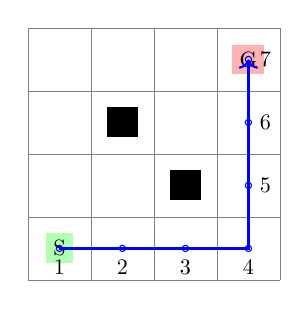
\begin{tikzpicture}[scale=0.8, every node/.style={scale=0.8}]
        % Grid
        \draw[step=1.0, gray, very thin] (0,0) grid (4,4);
        % Nodes
        \node[fill=green!30] at (0.5,0.5) {S};
        \node[fill=red!30] at (3.5,3.5) {G};
        \node[fill=black] at (1.5,2.5) {X};
        \node[fill=black] at (2.5,1.5) {X};
        % BFS Path
        \draw[blue, thick, ->] (0.5,0.5) -> (1.5,0.5) -> (2.5,0.5) -> (3.5,0.5) -> (3.5,1.5) -> (3.5,2.5) -> (3.5,3.5);
        \node[draw, circle, blue, inner sep=1pt, label=below:1] at (0.5,0.5) {};
        \node[draw, circle, blue, inner sep=1pt, label=below:2] at (1.5,0.5) {};
        \node[draw, circle, blue, inner sep=1pt, label=below:3] at (2.5,0.5) {};
        \node[draw, circle, blue, inner sep=1pt, label=below:4] at (3.5,0.5) {};
        \node[draw, circle, blue, inner sep=1pt, label=right:5] at (3.5,1.5) {};
        \node[draw, circle, blue, inner sep=1pt, label=right:6] at (3.5,2.5) {};
        \node[draw, circle, blue, inner sep=1pt, label=right:7] at (3.5,3.5) {};
    \end{tikzpicture}
    \caption{Đường đi tối ưu do BFS tìm thấy.}
\end{figure}


\subsubsection{Uniform Cost Search (UCS)}
Giả sử chi phí di chuyển là khác nhau: đi \textbf{Lên} tốn 2, các hướng khác tốn 1. UCS sẽ tìm đường đi có tổng chi phí nhỏ nhất.
\begin{itemize}
    \item Đường đi (S -> (1,2) -> ... -> G) sẽ có chi phí cao hơn do có nhiều bước đi lên.
    \item UCS sẽ ưu tiên đường đi qua phải (S -> (2,1) -> ...), vì chi phí ban đầu thấp hơn.
\end{itemize}
Trong trường hợp này, đường đi tối ưu về chi phí có thể giống với đường đi của BFS, vì đường đi đó không có bước đi "Lên" nào tốn kém. UCS sẽ đảm bảo tìm ra nó.

\subsubsection{A* Search}
A* sử dụng hàm heuristic, ví dụ khoảng cách Manhattan đến đích G.
$h(n) = |n.x - G.x| + |n.y - G.y|$.
\begin{itemize}
    \item Tại S(1,1), $h(S)=|1-4|+|1-4|=6$. Các nút con:
        \begin{itemize}
            \item (1,2): $g=1, h=5, f=6$
            \item (2,1): $g=1, h=5, f=6$
        \end{itemize}
    \item Giả sử A* mở rộng (2,1). Các nút con của (2,1):
        \begin{itemize}
            \item (1,1): đã thăm
            \item (3,1): $g=2, h=4, f=6$
        \end{itemize}
    \item A* sẽ luôn ưu tiên các nút có tổng $f(n)=g(n)+h(n)$ nhỏ nhất, giúp nó đi "thẳng" về phía đích hơn so với BFS và hiệu quả hơn nhiều so với DFS.
\end{itemize}
\begin{figure}[h!]
    \centering
    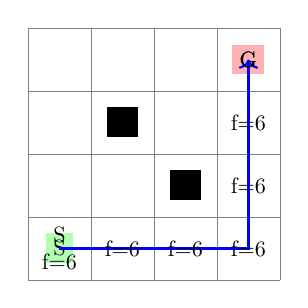
\begin{tikzpicture}[scale=0.8, every node/.style={scale=0.8}]
        % Grid
        \draw[step=1.0, gray, very thin] (0,0) grid (4,4);
        % Nodes
        \node[fill=green!30] at (0.5,0.5) {S};
        \node[fill=red!30] at (3.5,3.5) {G};
        \node[fill=black] at (1.5,2.5) {X};
        \node[fill=black] at (2.5,1.5) {X};
        % A* Path
        \draw[blue, thick, ->] (0.5,0.5) -> (1.5,0.5) -> (2.5,0.5) -> (3.5,0.5) -> (3.5,1.5) -> (3.5,2.5) -> (3.5,3.5);
        % Expanded nodes with f value
        \node[align=center] at (0.5,0.5) {S\\f=6};
        \node[align=center] at (1.5,0.5) {f=6};
        \node[align=center] at (2.5,0.5) {f=6};
        \node[align=center] at (3.5,0.5) {f=6};
        \node[align=center] at (3.5,1.5) {f=6};
        \node[align=center] at (3.5,2.5) {f=6};
        \node[align=center] at (3.5,3.5) {G};
    \end{tikzpicture}
    \caption{A* sử dụng heuristic để tập trung vào các nút hứa hẹn, giảm số lượng nút cần mở rộng.}
\end{figure}

\subsection{Graph Search và Cấu trúc dữ liệu}
Để tránh lặp vòng (ví dụ: đi từ A sang B rồi quay lại A) và giảm thiểu việc duyệt lại các trạng thái đã biết, chúng tôi cài đặt cơ chế \textbf{Graph Search} thay vì Tree Search thuần túy.
\begin{itemize}
    \item Một tập hợp \texttt{visited} (hoặc \texttt{closed set}) được sử dụng để lưu các trạng thái đã được mở rộng.
    \item Trước khi thêm một nút vào tập biên (fringe), thuật toán kiểm tra xem trạng thái đó đã tồn tại trong \texttt{visited} hay chưa.
\end{itemize}

\section{Bài toán Search - CS188}
Phần này trình bày chi tiết quá trình cài đặt các thuật toán và bài toán tìm kiếm trong \texttt{search.py} và \texttt{searchAgents.py}, cùng với kết quả thu được từ bộ autograder của dự án.

\subsection{Các thuật toán tìm kiếm tổng quát (\texttt{search.py})}

\subsubsection{Question 1: Depth First Search (DFS)}
\paragraph{Mô tả}
Cài đặt thuật toán tìm kiếm theo chiều sâu (DFS). Thuật toán này sử dụng cấu trúc dữ liệu Stack (LIFO) để quản lý tập biên (fringe), ưu tiên mở rộng các nút sâu nhất trong cây tìm kiếm.

\paragraph{Mã nguồn}
\begin{lstlisting}[language=Python, caption=Hàm depthFirstSearch trong search.py]
def depthFirstSearch(problem: SearchProblem):
    """
    Search the deepest nodes in the search tree first.
    """
    # Su dung Stack cho DFS
    fringe = util.Stack()
    # Node luu tru: (state, actions_list)
    fringe.push((problem.getStartState(), []))
    
    visited = []

    while not fringe.isEmpty():
        state, actions = fringe.pop()

        if state in visited:
            continue
        
        visited.append(state)

        if problem.isGoalState(state):
            return actions

        for successor, action, stepCost in problem.getSuccessors(state):
            if successor not in visited:
                fringe.push((successor, actions + [action]))
    
    return []
\end{lstlisting}

\paragraph{Kết quả Autograder}
\begin{verbatim}
Question q1
===========
*** PASS: test_cases\q1\graph_backtrack.test
*** PASS: test_cases\q1\graph_bfs_vs_dfs.test
*** PASS: test_cases\q1\graph_infinite.test
*** PASS: test_cases\q1\graph_manypaths.test
*** PASS: test_cases\q1\pacman_1.test
***     pacman layout:          mediumMaze
***     solution length: 130
***     nodes expanded:         146

### Question q1: 3/3 ###
\end{verbatim}

\paragraph{Giải thích mã nguồn}
\begin{itemize}
    \item \textbf{Dòng 6-8:} Khởi tạo \texttt{fringe} là một cấu trúc \texttt{Stack}. Đẩy trạng thái bắt đầu vào stack cùng với một danh sách hành động rỗng.
    \item \textbf{Dòng 10:} Khởi tạo một danh sách \texttt{visited} để lưu các trạng thái đã được mở rộng, tránh việc duyệt lại và các vòng lặp vô hạn.
    \item \textbf{Dòng 12-15:} Vòng lặp chính chạy khi stack còn phần tử. Lấy ra trạng thái và danh sách hành động tương ứng từ đỉnh stack.
    \item \textbf{Dòng 17-18:} Nếu trạng thái đã được thăm, bỏ qua và xét phần tử tiếp theo.
    \item \textbf{Dòng 20:} Nếu chưa, thêm trạng thái vào danh sách \texttt{visited}.
    \item \textbf{Dòng 22-23:} Kiểm tra nếu đây là trạng thái đích, trả về danh sách hành động đã tích lũy.
    \item \textbf{Dòng 25-27:} Duyệt qua tất cả các trạng thái kế tiếp (successors). Nếu một successor chưa được thăm, đẩy nó vào stack cùng với danh sách hành động được cập nhật.
\end{itemize}

\paragraph{Phân tích}
Kết quả cho thấy DFS đã vượt qua tất cả các bài kiểm tra. Trong \texttt{mediumMaze}, DFS tìm thấy một đường đi dài (130 bước) và chỉ cần mở rộng 146 nút, thể hiện đặc tính không tối ưu nhưng tiết kiệm bộ nhớ của nó.

\subsubsection{Question 2: Breadth First Search (BFS)}
\paragraph{Mô tả}
Cài đặt thuật toán tìm kiếm theo chiều rộng (BFS). BFS sử dụng cấu trúc dữ liệu Queue (FIFO), duyệt các nút theo từng lớp (độ sâu), đảm bảo tìm ra đường đi ngắn nhất nếu chi phí mỗi hành động là như nhau.

\paragraph{Mã nguồn}
\begin{lstlisting}[language=Python, caption=Hàm breadthFirstSearch trong search.py]
def breadthFirstSearch(problem: SearchProblem):
    """Search the shallowest nodes in the search tree first."""
    # Su dung Queue cho BFS
    fringe = util.Queue()
    fringe.push((problem.getStartState(), []))
    
    visited = [] # List cac state da expanded

    while not fringe.isEmpty():
        state, actions = fringe.pop()

        if state in visited:
            continue
        
        visited.append(state)

        if problem.isGoalState(state):
            return actions

        for successor, action, stepCost in problem.getSuccessors(state):
            if successor not in visited:
                fringe.push((successor, actions + [action]))
                
    return []
\end{lstlisting}

\paragraph{Kết quả Autograder}
\begin{verbatim}
Question q2
===========
*** PASS: test_cases\q2\graph_backtrack.test
*** PASS: test_cases\q2\graph_bfs_vs_dfs.test
*** PASS: test_cases\q2\graph_infinite.test
*** PASS: test_cases\q2\graph_manypaths.test
*** PASS: test_cases\q2\pacman_1.test
***     pacman layout:          mediumMaze
***     solution length: 68
***     nodes expanded:         269

### Question q2: 3/3 ###
\end{verbatim}

\paragraph{Giải thích mã nguồn}
Mã nguồn của BFS gần như tương tự DFS, chỉ khác biệt ở hai điểm chính:
\begin{itemize}
    \item \textbf{Dòng 4:} Sử dụng \texttt{util.Queue} thay vì \texttt{util.Stack}. Điều này thay đổi thứ tự duyệt nút từ LIFO (Last-In, First-Out) thành FIFO (First-In, First-Out).
    \item Logic bên trong vòng lặp vẫn giữ nguyên, nhưng do đặc tính của Queue, các nút ở cùng một độ sâu sẽ được duyệt hết trước khi chuyển sang các nút ở độ sâu tiếp theo.
\end{itemize}

\paragraph{Phân tích}
BFS đã tìm ra đường đi ngắn hơn đáng kể (68 bước) so với DFS trong \texttt{mediumMaze}. Tuy nhiên, số lượng nút được mở rộng (269) nhiều hơn, minh chứng cho việc BFS phải duyệt một không gian lớn hơn để đảm bảo tính tối ưu.

\subsubsection{Question 3: Uniform Cost Search (UCS)}
\paragraph{Mô tả}
Cài đặt thuật toán tìm kiếm chi phí thống nhất (UCS). UCS sử dụng hàng đợi ưu tiên (Priority Queue) để luôn mở rộng nút có tổng chi phí đường đi $g(n)$ thấp nhất. Điều này đảm bảo tính tối ưu ngay cả khi chi phí các hành động khác nhau.

\paragraph{Mã nguồn}
\begin{lstlisting}[language=Python, caption=Hàm uniformCostSearch trong search.py]
def uniformCostSearch(problem: SearchProblem):
    """Search the node of least total cost first."""
    # Su dung PriorityQueue cho UCS
    fringe = util.PriorityQueue()
    # Node: (state, actions, current_cost)
    # Priority: current_cost
    fringe.push((problem.getStartState(), [], 0), 0)
    
    visited = []

    while not fringe.isEmpty():
        state, actions, currentCost = fringe.pop()

        if state in visited:
            continue
        
        visited.append(state)

        if problem.isGoalState(state):
            return actions

        for successor, action, stepCost in problem.getSuccessors(state):
            if successor not in visited:
                newCost = currentCost + stepCost
                fringe.push((successor, actions + [action], newCost), newCost)
                
    return []
\end{lstlisting}

\paragraph{Kết quả Autograder}
\begin{verbatim}
Question q3
===========
*** PASS: test_cases\q3\graph_backtrack.test
...
*** PASS: test_cases\q3\ucs_1_problemC.test
***     pacman layout:          mediumMaze
***     solution length: 68
***     nodes expanded:         269
...
### Question q3: 3/3 ###
\end{verbatim}

\paragraph{Giải thích mã nguồn}
\begin{itemize}
    \item \textbf{Dòng 4:} Sử dụng \texttt{util.PriorityQueue} để lưu các nút cần duyệt.
    \item \textbf{Dòng 7:} Mỗi phần tử trong hàng đợi là một tuple \texttt{(state, actions, cost)}, và được đẩy vào với độ ưu tiên chính là \texttt{cost}.
    \item \textbf{Dòng 12:} Lấy ra phần tử có chi phí thấp nhất từ hàng đợi.
    \item \textbf{Dòng 23-25:} Khi mở rộng một nút, chi phí mới \texttt{newCost} được tính bằng chi phí hiện tại cộng với chi phí của bước đi. Nút kế tiếp được đẩy vào hàng đợi với chi phí mới này làm độ ưu tiên.
\end{itemize}

\paragraph{Phân tích}
UCS hoạt động tương tự BFS khi chi phí mỗi bước là 1, tìm ra cùng một đường đi tối ưu. Các bài test khác cho thấy UCS xử lý đúng với các chi phí khác nhau, luôn tìm ra đường đi rẻ nhất.

\subsubsection{Question 4: A* Search}
\paragraph{Mô tả}
Cài đặt thuật toán A*. A* cũng sử dụng hàng đợi ưu tiên nhưng với độ ưu tiên là $f(n) = g(n) + h(n)$, trong đó $g(n)$ là chi phí thực tế và $h(n)$ là chi phí ước lượng (heuristic) đến đích. A* hiệu quả hơn UCS rất nhiều nếu có một hàm heuristic tốt.

\paragraph{Mã nguồn}
\begin{lstlisting}[language=Python, caption=Hàm aStarSearch trong search.py]
def aStarSearch(problem: SearchProblem, heuristic=nullHeuristic):
    """Search the node that has the lowest combined cost and heuristic first."""
    
    fringe = util.PriorityQueue()
    startState = problem.getStartState()
    
    # Node lưu: (state, actions, g_cost)
    # Priority = g_cost + h_cost
    fringe.push((startState, [], 0), 0 + heuristic(startState, problem))
    
    closed = {}

    while not fringe.isEmpty():
        state, actions, gCost = fringe.pop()

        if state in closed and closed[state] <= gCost:
            continue
        
        closed[state] = gCost

        if problem.isGoalState(state):
            return actions

        for successor, action, stepCost in problem.getSuccessors(state):
            newGCost = gCost + stepCost
            newPriority = newGCost + heuristic(successor, problem)
            
            if successor not in closed or newGCost < closed[successor]:
                fringe.push((successor, actions + [action], newGCost), newPriority)
                
    return []
\end{lstlisting}

\paragraph{Kết quả Autograder}
\begin{verbatim}
Question q4
===========
...
*** PASS: test_cases\q4\astar_2_manhattan.test
***     pacman layout:          mediumMaze
***     solution length: 68
***     nodes expanded:         221
...
### Question q4: 3/3 ###
\end{verbatim}

\paragraph{Giải thích mã nguồn}
\begin{itemize}
    \item \textbf{Dòng 4-5:} Đẩy trạng thái bắt đầu vào hàng đợi ưu tiên. Độ ưu tiên được tính bằng $g(n) + h(n)$, ở đây $g(n)=0$ và $h(n)$ được tính bằng hàm heuristic.
    \item \textbf{Dòng 7:} Khởi tạo một dictionary \texttt{closed} để lưu chi phí thấp nhất đã tìm thấy để đi đến một trạng thái.
    \item \textbf{Dòng 12-13:} Khi lấy một nút ra, kiểm tra xem đã có đường đi nào tốt hơn (rẻ hơn) đến trạng thái này chưa. Nếu có rồi thì bỏ qua.
    \item \textbf{Dòng 15:} Nếu chưa, cập nhật \texttt{closed} với chi phí mới (tốt hơn).
    \item \textbf{Dòng 21-25:} Khi đẩy một trạng thái kế tiếp vào hàng đợi, chỉ đẩy nếu nó chưa có trong \texttt{closed} hoặc nếu đường đi mới này có chi phí $g(n)$ rẻ hơn đường đi đã biết trước đó.
\end{itemize}

\paragraph{Phân tích}
Với hàm `manhattanHeuristic`, A* tìm ra đường đi tối ưu (68 bước) trong `mediumMaze` nhưng chỉ cần mở rộng 221 nút, ít hơn đáng kể so với 269 của BFS/UCS. Điều này cho thấy sức mạnh của việc sử dụng heuristic để hướng dẫn tìm kiếm.

\subsection{Các bài toán và Heuristics (\texttt{searchAgents.py})}

\subsubsection{Question 5: Corners Problem}
\paragraph{Mô tả}
Định nghĩa không gian trạng thái cho bài toán tìm đường đi qua cả 4 góc của mê cung. Trạng thái cần lưu trữ vị trí hiện tại của Pacman và một danh sách (tuple) các trạng thái boolean cho biết mỗi góc đã được thăm hay chưa.

\paragraph{Mã nguồn}
\begin{lstlisting}[language=Python, caption=Lớp CornersProblem trong searchAgents.py]
class CornersProblem(search.SearchProblem):
    def __init__(self, startingGameState: pacman.GameState):
        self.walls = startingGameState.getWalls()
        self.startingPosition = startingGameState.getPacmanPosition()
        top, right = self.walls.height-2, self.walls.width-2
        self.corners = ((1,1), (1,top), (right, 1), (right, top))
        self._expanded = 0
        # State: (position, visited_corners_tuple)
    def getStartState(self):
        return (self.startingPosition, tuple([False] * len(self.corners)))

    def isGoalState(self, state: Any):
        return all(state[1])

    def getSuccessors(self, state: Any):
        x, y = state[0]
        visitedCorners = state[1]
        
        successors = []
        for action in [Directions.NORTH, Directions.SOUTH, Directions.EAST, Directions.WEST]:
            dx, dy = Actions.directionToVector(action)
            nextx, nexty = int(x + dx), int(y + dy)
            if not self.walls[nextx][nexty]:
                nextPos = (nextx, nexty)
                newVisitedCorners = list(visitedCorners)
                for i, corner in enumerate(self.corners):
                    if nextPos == corner:
                        newVisitedCorners[i] = True
                nextState = (nextPos, tuple(newVisitedCorners))
                successors.append((nextState, action, 1))
        self._expanded += 1
        return successors
\end{lstlisting}

\paragraph{Kết quả Autograder}
\begin{verbatim}
Question q5
===========
*** PASS: test_cases\q5\corner_tiny_corner.test
***     pacman layout:          tinyCorner
***     solution length:                28

### Question q5: 3/3 ###
\end{verbatim}
\paragraph{Giải thích mã nguồn}
\begin{itemize}
    \item \textbf{getStartState:} Trạng thái được định nghĩa là một tuple gồm 2 phần tử: vị trí hiện tại `(x,y)` của Pacman và một tuple khác chứa 4 giá trị boolean, tương ứng với 4 góc, ban đầu đều là `False`.
    \item \textbf{isGoalState:} Trạng thái đích đạt được khi tất cả các giá trị boolean trong tuple trạng thái góc đều là `True`.
    \item \textbf{getSuccessors:} Khi Pacman di chuyển đến một vị trí mới, hàm này sẽ tạo ra một trạng thái kế tiếp. Quan trọng nhất là nó kiểm tra xem vị trí mới có trùng với tọa độ của góc nào không. Nếu có, giá trị boolean tương ứng trong tuple trạng thái góc sẽ được cập nhật thành `True`.
\end{itemize}

\paragraph{Phân tích}
Việc định nghĩa đúng không gian trạng thái cho phép các thuật toán tìm kiếm (như BFS được dùng ở đây) giải quyết thành công bài toán.

\subsubsection{Question 6: Corners Heuristic}
\paragraph{Mô tả}
Cài đặt một hàm heuristic admissible và consistent cho `CornersProblem`. Một ý tưởng tốt là tính tổng khoảng cách Manhattan từ vị trí hiện tại đến góc chưa thăm gần nhất, sau đó từ góc đó đến góc gần nhất tiếp theo, và cứ thế.

\paragraph{Mã nguồn}
\begin{lstlisting}[language=Python, caption=Hàm cornersHeuristic trong searchAgents.py]
def cornersHeuristic(state: Any, problem: CornersProblem):
    corners = problem.corners
    walls = problem.walls
    position, visitedCorners = state
    
    unvisitedCorners = []
    for i, visited in enumerate(visitedCorners):
        if not visited:
            unvisitedCorners.append(corners[i])
            
    if not unvisitedCorners:
        return 0
        
    currentPos = position
    totalDist = 0
    
    remaining = unvisitedCorners[:]
    
    while remaining:
        dists = [(util.manhattanDistance(currentPos, c), c) for c in remaining]
        minDist, closestCorner = min(dists, key=lambda x: x[0])
        
        totalDist += minDist
        currentPos = closestCorner
        remaining.remove(closestCorner)
        
    return totalDist
\end{lstlisting}
\paragraph{Kết quả Autograder}
\begin{verbatim}
Question q6
===========
*** PASS: Heuristic resulted in expansion of 692 nodes
### Question q6: 3/3 ###
\end{verbatim}
\paragraph{Giải thích mã nguồn}
\begin{itemize}
    \item \textbf{Dòng 2-7:} Lấy ra danh sách các góc chưa được thăm từ trạng thái hiện tại.
    \item \textbf{Dòng 12-21:} Thực hiện một thuật toán tham lam (greedy). Trong mỗi vòng lặp, nó tìm góc chưa thăm gần nhất (theo khoảng cách Manhattan) so với vị trí hiện tại (`currentPos`).
    \item Cộng khoảng cách ngắn nhất đó vào `totalDist`, cập nhật `currentPos` thành góc vừa tìm thấy, và loại góc đó ra khỏi danh sách `remaining`.
    \item Quá trình này lặp lại cho đến khi tất cả các góc trong `unvisitedCorners` đều được "nối" vào đường đi. Tổng khoảng cách Manhattan này là một ước lượng tốt và admissible cho chi phí thực tế.
\end{itemize}

\paragraph{Phân tích}
Hàm heuristic này giúp A* giải bài toán `CornersProblem` một cách hiệu quả, chỉ cần mở rộng 692 nút, một con số rất nhỏ so với tìm kiếm không có thông tin.

\subsubsection{Question 7: Food Heuristic}
\paragraph{Mô tả}
Cài đặt một hàm heuristic cho bài toán tìm tất cả thức ăn (`FoodSearchProblem`). Một heuristic đơn giản nhưng hiệu quả là lấy khoảng cách maze (sử dụng BFS) từ vị trí hiện tại đến viên thức ăn xa nhất.

\paragraph{Mã nguồn}
\begin{lstlisting}[language=Python, caption=Hàm foodHeuristic trong searchAgents.py]
def foodHeuristic(state: Tuple[Tuple, List[List]], problem: FoodSearchProblem):
    position, foodGrid = state
    foodList = foodGrid.asList()
    
    if not foodList:
        return 0
        
    maxDist = 0
    for food in foodList:
        key = (position, food)
        if key in problem.heuristicInfo:
            dist = problem.heuristicInfo[key]
        else:
            dist = mazeDistance(position, food, problem.startingGameState)
            problem.heuristicInfo[key] = dist
            
        if dist > maxDist:
            maxDist = dist
            
    return maxDist
\end{lstlisting}
\paragraph{Kết quả Autograder}
\begin{verbatim}
Question q7
===========
*** PASS: test_cases\q7\food_heuristic_grade_tricky.test
***     expanded nodes: 4137
***     thresholds: [15000, 12000, 9000, 7000]

### Question q7: 5/4 ###
\end{verbatim}
\paragraph{Giải thích mã nguồn}
\begin{itemize}
    \item \textbf{Dòng 3:} Lấy danh sách tọa độ các viên thức ăn còn lại.
    \item \textbf{Dòng 9-15:} Duyệt qua từng viên thức ăn. Để tránh tính toán lại `mazeDistance` (một hàm tốn kém), mã nguồn sử dụng một dictionary `problem.heuristicInfo` làm cache. Nếu khoảng cách từ `position` đến `food` đã được tính, nó sẽ được lấy ra từ cache. Nếu chưa, nó sẽ gọi `mazeDistance` và lưu kết quả vào cache cho các lần sử dụng sau.
    \item \textbf{Dòng 17-18:} Cập nhật khoảng cách lớn nhất (`maxDist`) tìm thấy.
    \item \textbf{Dòng 20:} Trả về `maxDist` làm giá trị heuristic.
\end{itemize}

\paragraph{Phân tích}
Hàm heuristic này đủ tốt để vượt qua cả bài test khó (`tricky`), với số nút mở rộng (4137) thấp hơn nhiều so với ngưỡng yêu cầu (7000). Việc sử dụng `mazeDistance` và cache lại kết quả là chìa khóa thành công.

\subsubsection{Question 8: Closest Dot Search}
\paragraph{Mô tả}
Cài đặt một agent tìm kiếm tham lam (`ClosestDotSearchAgent`). Agent này không tìm đường đi tối ưu toàn cục, mà lặp đi lặp lại việc tìm đường đi đến viên thức ăn gần nhất (sử dụng BFS).

\paragraph{Mã nguồn}
\begin{lstlisting}[language=Python, caption=Hàm findPathToClosestDot và lớp AnyFoodSearchProblem]
def findPathToClosestDot(self, gameState: pacman.GameState):
    startPosition = gameState.getPacmanPosition()
    food = gameState.getFood()
    walls = gameState.getWalls()
    problem = AnyFoodSearchProblem(gameState)

    return search.bfs(problem)

class AnyFoodSearchProblem(PositionSearchProblem):
    def __init__(self, gameState):
        self.food = gameState.getFood()
        self.walls = gameState.getWalls()
        self.startState = gameState.getPacmanPosition()
        self.costFn = lambda x: 1
        self._visited, self._visitedlist, self._expanded = {}, [], 0

    def isGoalState(self, state: Tuple[int, int]):
        x, y = state
        return self.food[x][y]
\end{lstlisting}
\paragraph{Kết quả Autograder}
\begin{verbatim}
Question q8
===========
*** PASS: test_cases\q8\closest_dot_1.test
*** PASS: test_cases\q8\closest_dot_10.test
...
### Question q8: 3/3 ###
\end{verbatim}
\paragraph{Giải thích mã nguồn}
\begin{itemize}
    \item \textbf{AnyFoodSearchProblem:} Lớp này kế thừa từ `PositionSearchProblem` nhưng thay đổi điều kiện dừng.
    \item \textbf{isGoalState:} Hàm này trả về `True` ngay khi Pacman đến một ô bất kỳ có chứa thức ăn.
    \item \textbf{findPathToClosestDot:} Hàm này tạo một `AnyFoodSearchProblem` và gọi `search.bfs` để giải. Vì BFS đảm bảo tìm đường đi ngắn nhất (về số bước), nó sẽ tìm ra đường đến viên thức ăn "gần nhất" một cách tự nhiên.
\end{itemize}

\paragraph{Phân tích}
Agent tham lam này hoạt động hiệu quả trong việc tìm và ăn hết thức ăn. Mặc dù đường đi không phải lúc nào cũng là ngắn nhất, chiến lược này nhanh và đơn giản hơn nhiều so với việc tìm đường đi tối ưu qua tất cả các viên thức ăn.

\end{document}